%Custom Functions
\newcommand{\CompanyName}{TT} % update later

\documentclass[conference]{IEEEtran}
\IEEEoverridecommandlockouts
% The preceding line is only needed to identify funding in the first footnote. If that is unneeded, please comment it out.
%\usepackage{cite}
\usepackage{amsmath,amssymb,amsfonts}
\usepackage{algorithmic}
\usepackage{graphicx}
\usepackage{textcomp}
\usepackage{xcolor}

\usepackage{pdflscape}

\usepackage[utf8]{inputenc}
\usepackage{fancyhdr}
\usepackage{lastpage}

% Please add the following required packages to your document preamble:
\usepackage{multirow, makecell, rotating}
\usepackage[numbers]{natbib}

\usepackage{listings}
\usepackage{hyperref}
\usepackage{amsmath}


\hypersetup{
    citecolor=black,
    colorlinks=true,
    linkcolor=black,
    filecolor=magenta,      
	urlcolor=cyan
}

\usepackage{listings}
\usepackage{color}

\definecolor{dkgreen}{rgb}{0,0.6,0}
\definecolor{gray}{rgb}{0.5,0.5,0.5}
\definecolor{mauve}{rgb}{0.58,0,0.82}

\lstset{frame=single,
  language=C++,
  showstringspaces=false,
  columns=flexible,
  basicstyle={\small\ttfamily},
  numbers = none,
  numberstyle=\tiny\color{gray},
  keywordstyle=\color{blue},
  commentstyle=\color{dkgreen},
  stringstyle=\color{mauve},
  breaklines=true,
  breakatwhitespace=true,
  tabsize=2
}

\def\BibTeX{{\rm B\kern-.05em{\sc i\kern-.025em b}\kern-.08em
T\kern-.1667em\lower.7ex\hbox{E}\kern-.125emX}}

\fancypagestyle{fancylandscape}{
\fancyhf{} %Clears the header/footer
\fancyfoot{% Footer
\makebox[\textwidth][r]{% Right
  \rlap{\hspace{.75cm}% Push out of margin by \footskip
    \smash{% Remove vertical height
      \raisebox{4.87in}{% Raise vertically
        \rotatebox{90}{Page \thepage\ of \pageref{LastPage}}}}}}}% Rotate counter-clockwise
\renewcommand{\headrulewidth}{0pt}% No header rule
\renewcommand{\footrulewidth}{0pt}% No footer rule
}

\pagestyle{fancyplain}
\fancyhf{}
\fancyfoot[c]{Page \thepage\ of \pageref{LastPage}}
\renewcommand{\headrulewidth}{0pt}

\begin{document}

\title{A Risky Coexistence: Examining the Challenges Faced by Autonomous Vehicles and Motorcycles}

\author{\IEEEauthorblockN{1\textsuperscript{st} Given Edward Patch}
	\IEEEauthorblockA{\textit{Software Engineering and Artificial Intelligence (of MSc Year 4)} \\
		\textit{Autonomous Vehicle Research}\\
		\textit{University of Wales Trinity St. Davids (of Dr. Tim Bashford)}\\
		Swansea, Wales \\
		Student ID: 1801492}}

\maketitle
\thispagestyle{plain}
\pagestyle{plain}

\begin{abstract}

\end{abstract}

\begin{IEEEkeywords}
	Artificial Neural Networks, Autonomous Vehicles, 
\end{IEEEkeywords}

\section{Introduction}
	 Autonomous Vehicles (AVs) are scheduled to roll out to the United Kingdom roads by 2025.~\cite{govuk_self-driving_2022} With the rise of automated vehicles, a safety concern arises, which affects the development of AVs, including government bodies and manufacturers, public safety and the National Health Service (NHS), when it comes to motorcycles and AVs. The research focuses on issues that may have been overlooked already with motorcycles, with new scenarios introduced in many US states, like road widths, filtering and poor weather conditions with British vehicles. 

	Addressing these issues could be problematic; however, with Object Classification, which is not entirely accurate compared to AV standard, the research could push more extensive research in this area. The study's objectives are to understand the existing dangers with AVs and motorcycles, establish appropriate datasets to train and test the selected models, remove any vehicles that are not necessary for the study, and evaluate the test results of the study.
	
	A few study results are showcased to illustrate the current issues that may arise, describing the reasoning the model may have not detected. These results will be cross-referenced to research that did similar tests to support the argument to drive the safety issues that may still exist with AV manufacturers or newly established UK AV manufacturers.

\section{Literature Review}
	\subsection{Autonmous Vehicle Paradigm}
		An `intelligent vehicles' paradigm has three logical rule statements to follow. Firstly, the system will collect data from the driver, developing the knowledge from itself and the driver. Second, the system will have to perform some judgement. Silviu Ionita~\cite{ionita_autonomous_2017} mentions that it is paramount to filter the data through logical statements and apply multivalent logic to handle uncertainty better, creating a better judgement. ADAS require consistent autonomous behaviour to collect and handle the data even when the system is not in control. This behaviour means that the developers can collect data on what the system would have done if it were in control, allowing any refinement down the line and enabling AVs to work more efficiently.

		Figure~\ref{fig:adasFunctionsIonita} provides the structure of Advanced Driver Assistance Systems (ADAS) functions linking the responsibilities to the decision and action. Strategic Processes are near real-time, Tactical Processes are real-time, and Direct are short as possible. These three functionalities are fundamental when understanding how an ADAS vehicle copes and how an AV will tend to handle situations.~\cite{ionita_autonomous_2017} It is necessary to establish that the AV will only rely on its judgement after the decision to remove human interaction. Some of these system paradigms reflect the capabilities of AVs involving blindspots, low-light and poor weather conditions.
		\begin{figure}[h]
			\centering
			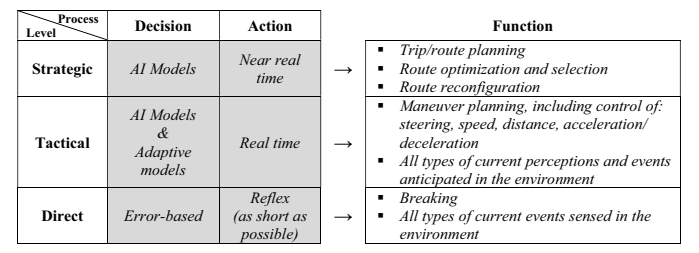
\includegraphics[width=\columnwidth]{Figures/SystemFunctionality-3.png}
			\caption{Classes of ADAS and their Requirements for Decision and Execution~\cite{ionita_autonomous_2017}}
			\label{fig:adasFunctionsIonita}
		\end{figure}

	\subsection{Vision Technology and Techniques}
		When investigating how AVs handle blindspot handling compared to human drivers, the paper `Automated driving: Safety blind spots' by Ian Y. Noy~\cite{noy_automated_2018} suggests the current implementations within ADAS and compares it to standard driving errors. Although, the paper does not directly reflect on motorcycles, the paper details ADAS systems and how the transition from ADAS to AVs is possible. An important quote from the paper is that `AD technologies are suboptimal in that they fail to address critical blind spots and will likely lead to unnecessary losses and injuries because insufficient consideration is given to integrating the human element into overall sociotechnical road transportation system'~\cite{noy_automated_2018} suggests that transitioning from ADAS to AVs is relatively dangerous if blindspot judgements are overlooked. With further research in this area, it will provide more information to understand if AVs are safer than human drivers on the road.

		Light Detection and Ranging (LiDAR) uses a pulsed laser to gather information about the object surroundings, providing depth that images cannot capture. Within the paper, `Pedestrian recognition and tracking using 3D LiDAR for autonomous vehicle' by Heng Wang~\cite{wang_pedestrian_2017}, a quote ``LiDARs are another kind of commonly used sensors for pedestrian recognition, compared with cameras, LiDARs can provide accurate range information and larger field of view.''. Heng Wang points out that the use of LiDAR widens the field of view.
		
		After researching some extra information, it was found within the report `What Happens for a ToF LiDAR in Fog?'~\cite{li_what_2021} that the failure rate of detection is Diffuse Reflection Targets: 2.1\% and Retro-Reflective Objects: 0.7\% in the range of 0-10m, Diffuse Reflection Targets: 10.3\% and Retro-Reflective Objects: 1.1\% in the range of 10-15m, Diffuse Reflection Targets: 15.1\% and Retro-Reflective Objects: 1.1\% in the range of 15-20m, and Diffuse Reflection Targets: 19.5\% and Retro-Reflective Objects: 0.7\% in the range of 0-10m~\cite{royo_overview_2019}

\section{Methodology}
	\subsection{Research Hypothesis}
		These hypothesis statements assist the explore the research question, `Are AVs a Danger to Motorcycles?':

		\begin{enumerate}
		\item Motorcycles have blindspots that are often overlooked by human drivers, which AVs can detect and avoid.
		\item In low light conditions, AVs may struggle to accurately detect and identify motorcycles, leading to potential safety issues on the road.
		\item Poor weather conditions, such as heavy rain, snow, or fog, can make it difficult for AVs to detect and react to motorcycles, increasing the risk of accidents.
		\end{enumerate}

	\subsection{Objectives}
	The main objectives of this project are to develop an accurate FER model using CNNs and to improve the model's performance on specific tasks. The following steps be undertaken to achieve these objectives:-

	\begin{enumerate}
		\item Dataset Preparation: Object Classification requires a set of labels to correspond to an image, mapping different classified objects wihin the image. Preparation of the data requires being able to select validated data for training and testing purposes.
		\item Pre-processing: Read in the mapping datasets and extract the sorted datasets to the designated file paths. 
		\item Architecture Selection and Optimisation: Investigate different object classification architectures, and select a model that could cloisely demonstrate an idea of how Autonomous Vehicles currently initialise object classification.
		\item Evaluation Techniques: A few methods to analyse and evaluate the model's performance and accuracy regarding the learning and predictive classifications. Classification Reports and Confusion Matrices to identify optimisation issues to improve accuracy results. Training and validation evaluation methods are required to determine the model's learning quality. The Python libraries involved includes history when a model is fitted, which includes `loss' and `val\_loss' to determine the optimisation of the learning state of the model. An evaluation of validation data is essential to highlight any errors within the preparation phase.
	\end{enumerate}

	\subsection{Sourcing and Preparation}
		The datasets being used are arranged in YOLOv7 format and would require additional modifications to work before the training phase. The datasets that have been decided to train the models are `Motorcycle Samples - v1 VMT-V1', sourced from Roboflow~\cite{roboflow_motorcycle_nodate}, and `Road Vehicle Images Dataset', sourced from Kaggle, authored by Ashfak Yeafi~\cite{ashfak_yeafi_road_nodate}.

		The training materials are split into `images' and `labels' categories, which require some preparation. Using Python scripts, the selected training material is taken and processed together, allowing the model to see different motorcycles in different scenarios. A US and Indian dataset was used to get other road conditions and various types of motorcycles. Using the two datasets helped increase the accuracy during the validation process. The materials are separated and combined into a CSV file format, and another Python Snippet can reconstruct the CSV and Image Data into a new directory.

	\subsection{Pre-Processing}
	\label{subsec:preprocessing}
		Training of two datasets, dataset A with the filter of `bus', `car', `minivan', `motorcycle', `pickup', `scooter', `trike', `truck', `van', `person', whereas dataset B involves; `motorcycle', `tricycle' and `person' filters. The `yolov5s.pts' and `yolov5l.pts' were used during testing, with better results on the `yolov5l.pts' by 25\% when identifying motorcycles. Both weights used a batch of thirty-two and ten epochs.

		Testing materials must include video content, split into multiple frames To test the trained YOLO model, with enough images to create a strong argument. Joining a motorcycle group and exploring various routes across the United Kingdom, including motorways, dual carriageways, A-roads, and backroads, with motorcycles overtaking, filtering, and navigating blindspots, can lead to unexplored scenarios and questions that may have been previously overlooked.
					
		A decided factor is to use a Drift Innovation Ghost XL motorcycle camera attached to a motorcycle that rides within the group, then swap the camera with another rider after some time. This way, combining the content helps identify how Object Classification copes with numerous blindspots and draws some questions to further the research concerning the current safety of AV vehicles. 
		
		One sports bike and two cruisers are selected for material to test how Object Classification models handle different motorcycle styles. Ideal footage would include Scramblers, Trikes and other similar vehicles to establish how Object Classification models work in an estimated manner. A perfect material would be that during the ride out, conducted on 18$^\text{th}$ July 2023, Tuesday, would capture these vehicles, which either pass by or join us in sections of the rides. The group is instructed to overtake and be undertaken by the camera vehicle to create plenty of footage to put the YOLO model to the test. However, it is worth noting that no rider is pressured into doing anything illegal or unsafe.

	\subsection{Model Architecture}
		With the challenge of setting up a high-end model equivalent to a leading AV manufacturer like Tesla, it is essential to use detailed Object Classification training material. Using the Qualitative Research method with video frames and labels to classify the different objects in the video is required. Roboflow and other materials are outsourced and looked into using different sources found in various research journals.

		Using Qualitative Research methods enhances the development of engaging with better architecture concepts. These give us a broad understanding of 

\section{Training Results}
		\begin{figure}[h]
			\centering
			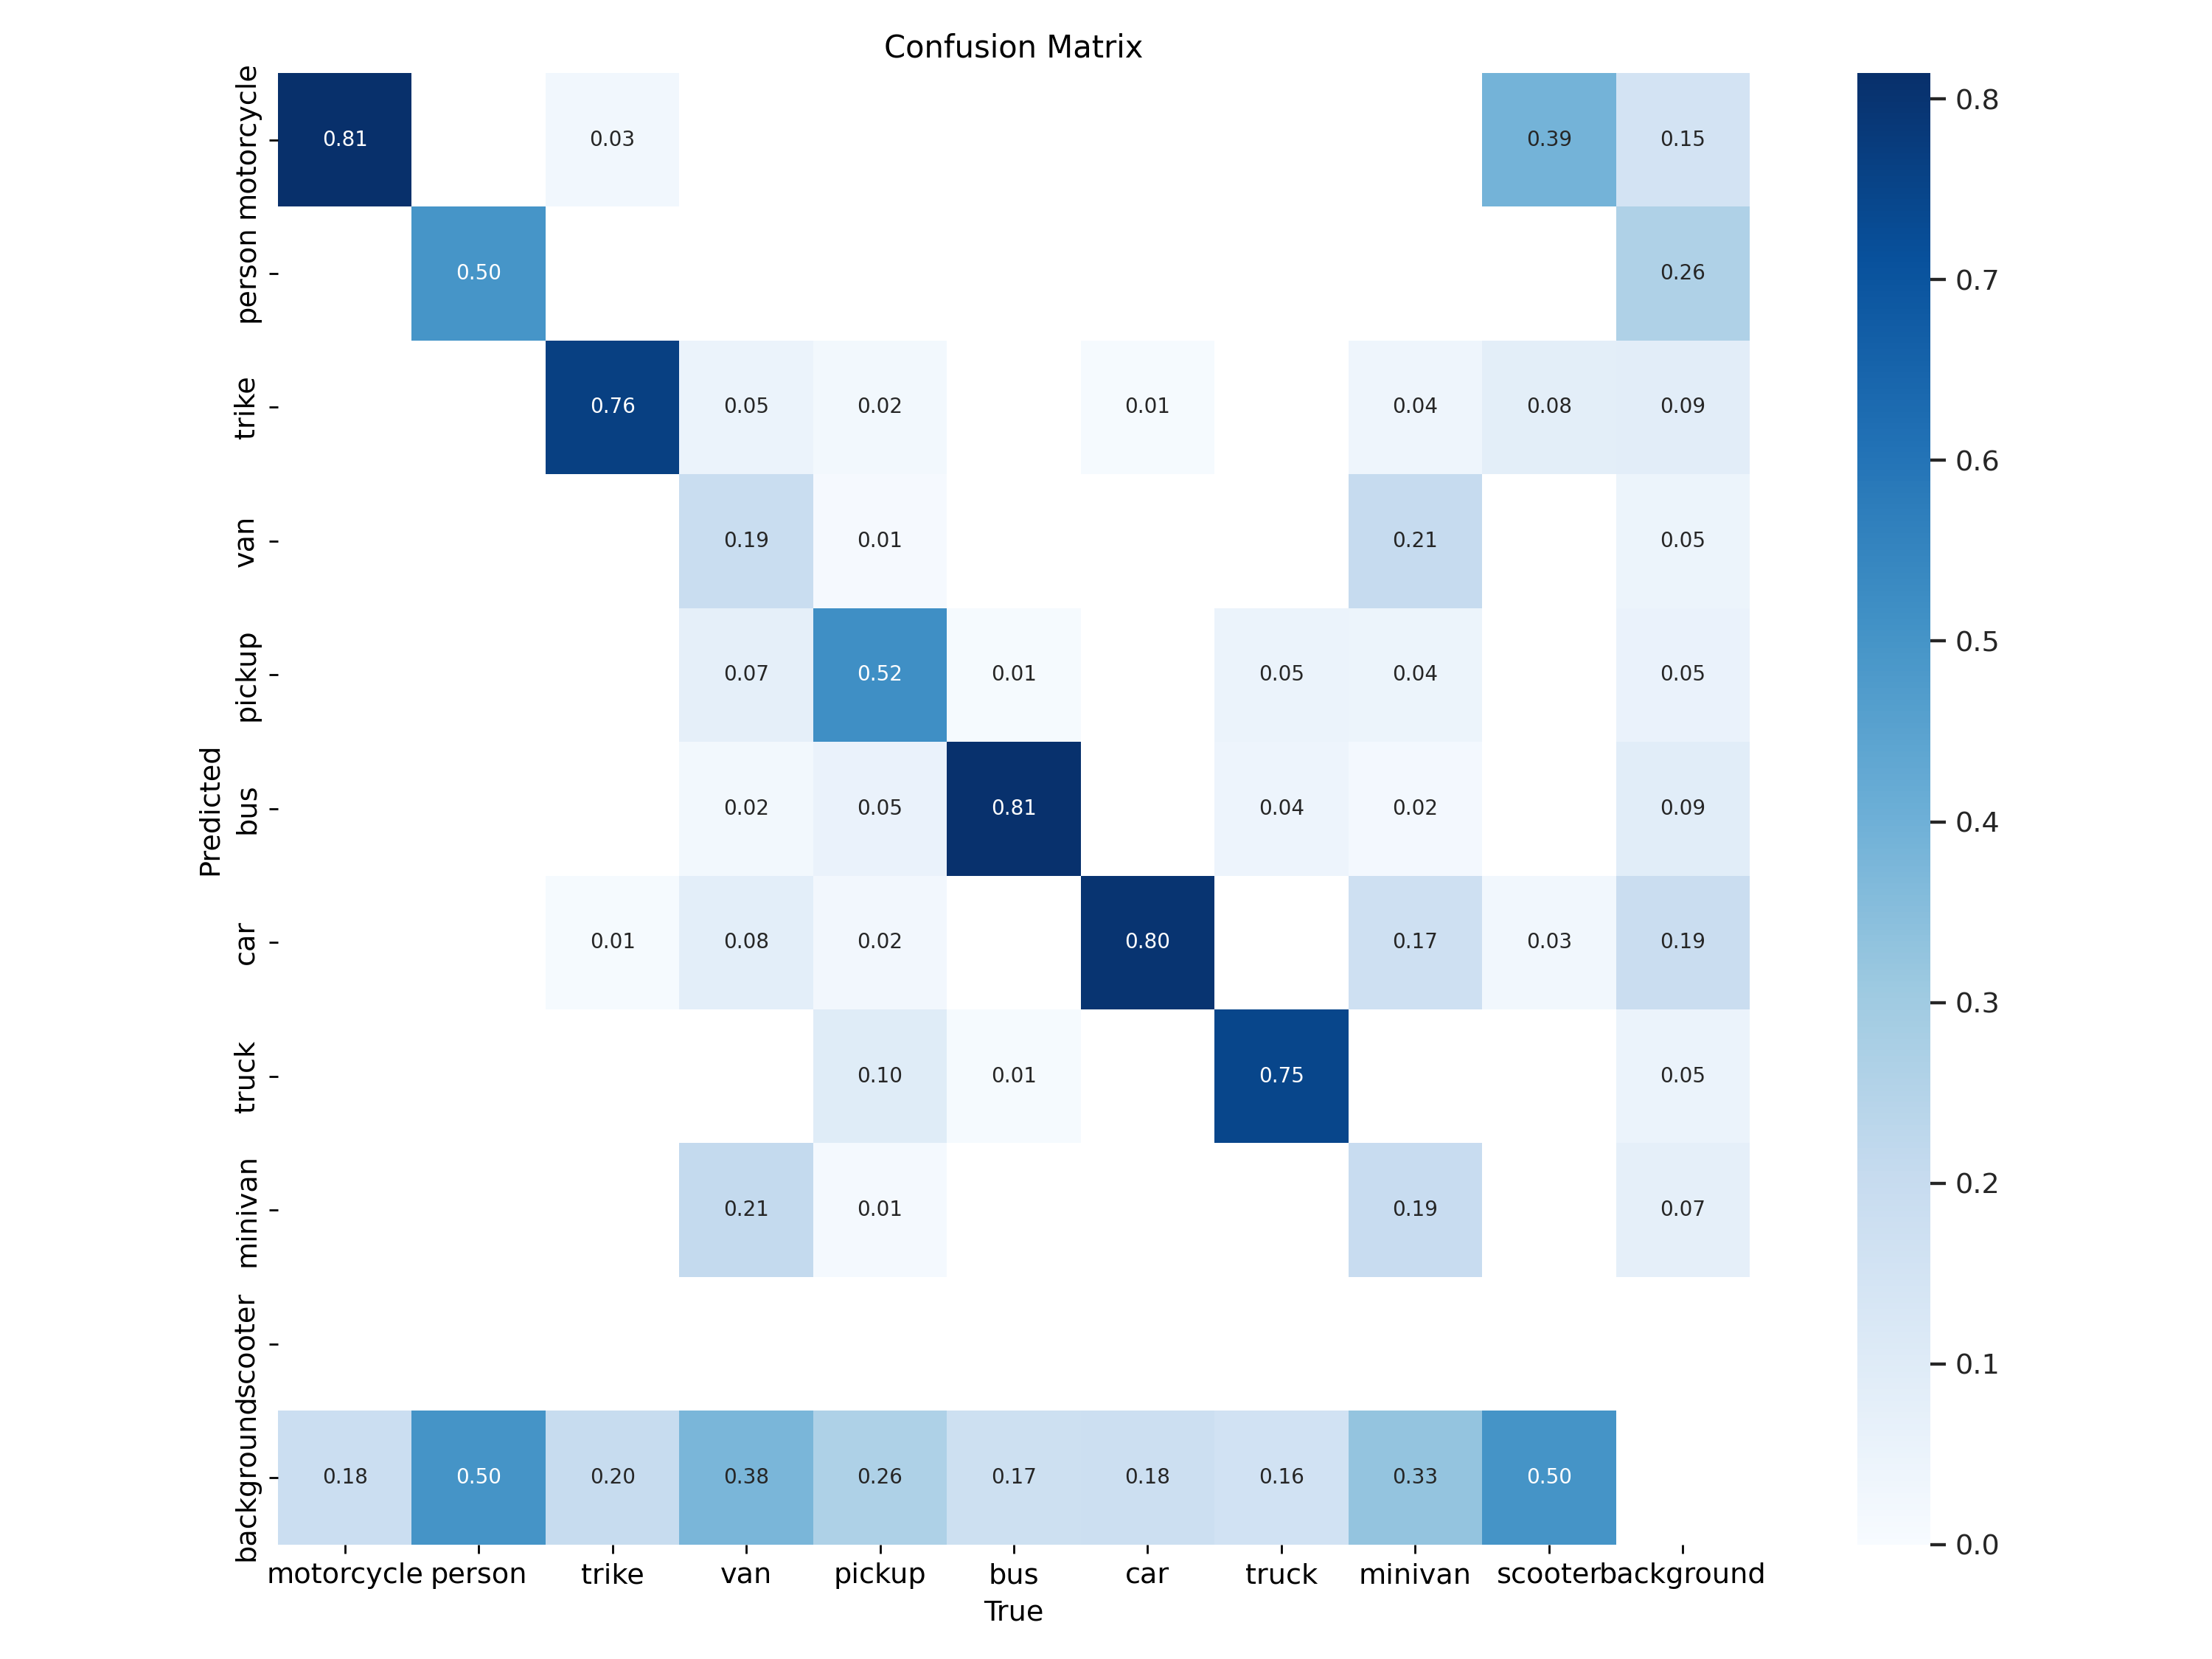
\includegraphics[width=\columnwidth]{Figures/dataset_a/a_confusion_matrix.png}
			\caption{Dataset A: Confusion Matrix of YOLOv5 model}
			\label{fig:ukDatasetYolov5LargeWeight}
		\end{figure}
		
		\begin{figure}[h]
			\centering
			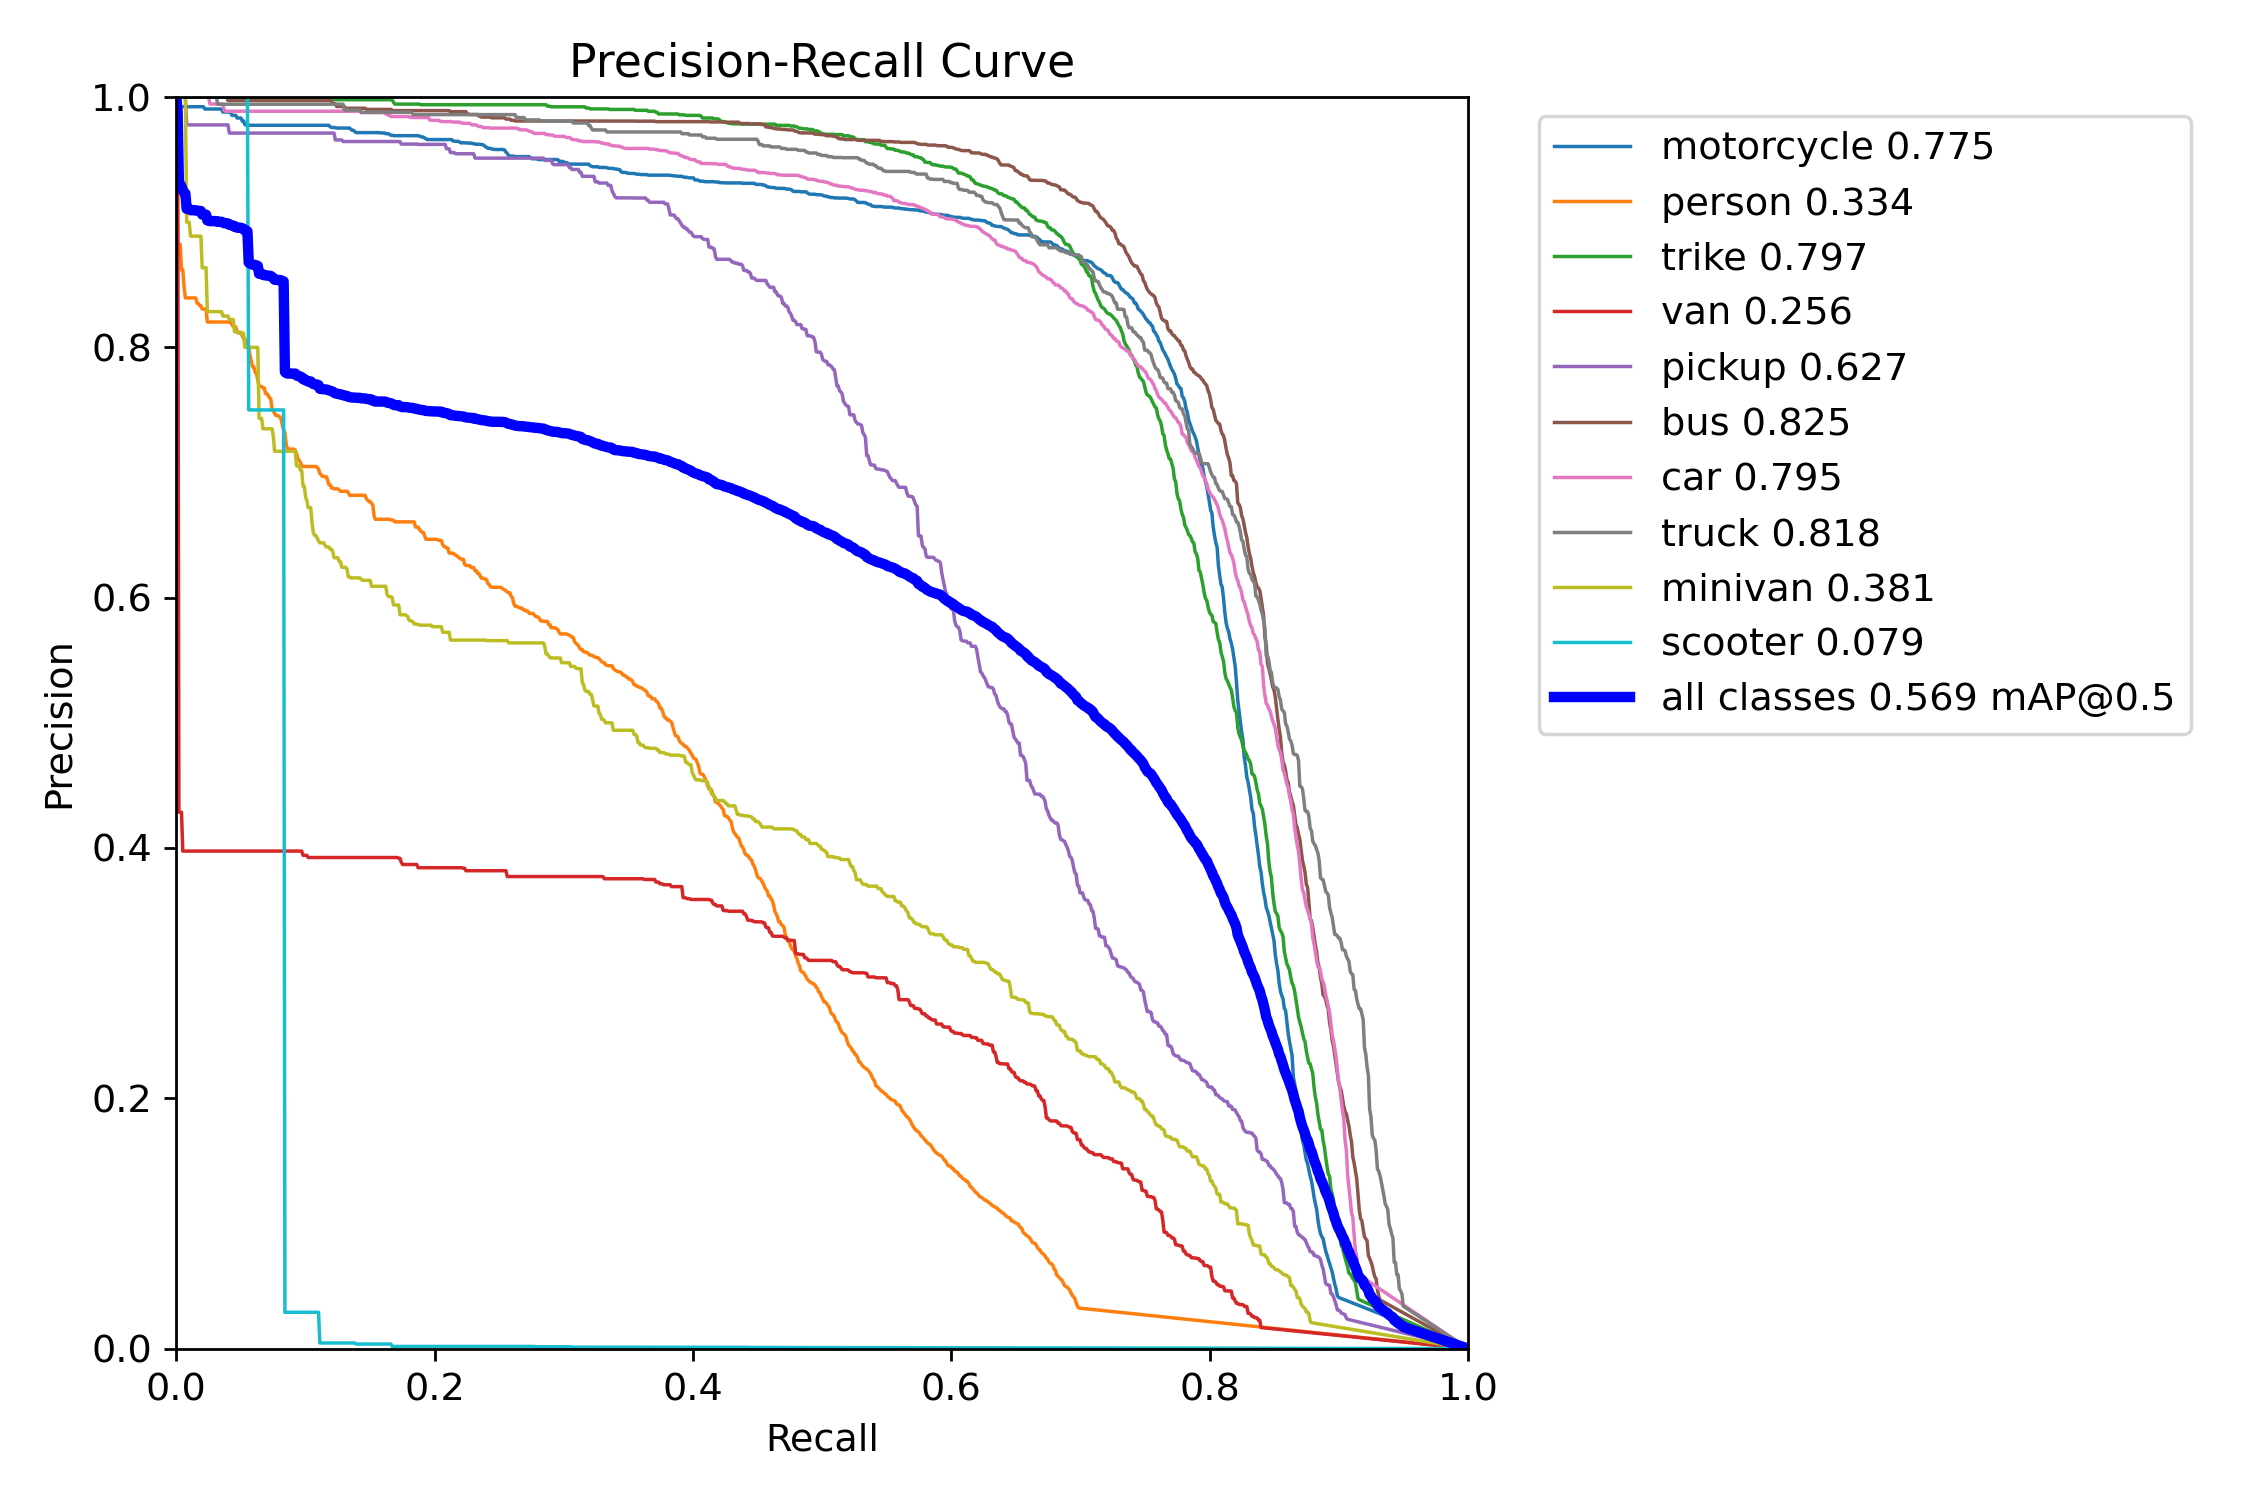
\includegraphics[width=\columnwidth]{Figures/dataset_a/PR_curve.png}
			\caption{Dataset A: Performance and Recall Curve of YOLOv5 model}
			\label{fig:ukDatasetYolov5LargeWeightPRCurve}
		\end{figure}

		\begin{figure}[h]
			\centering
			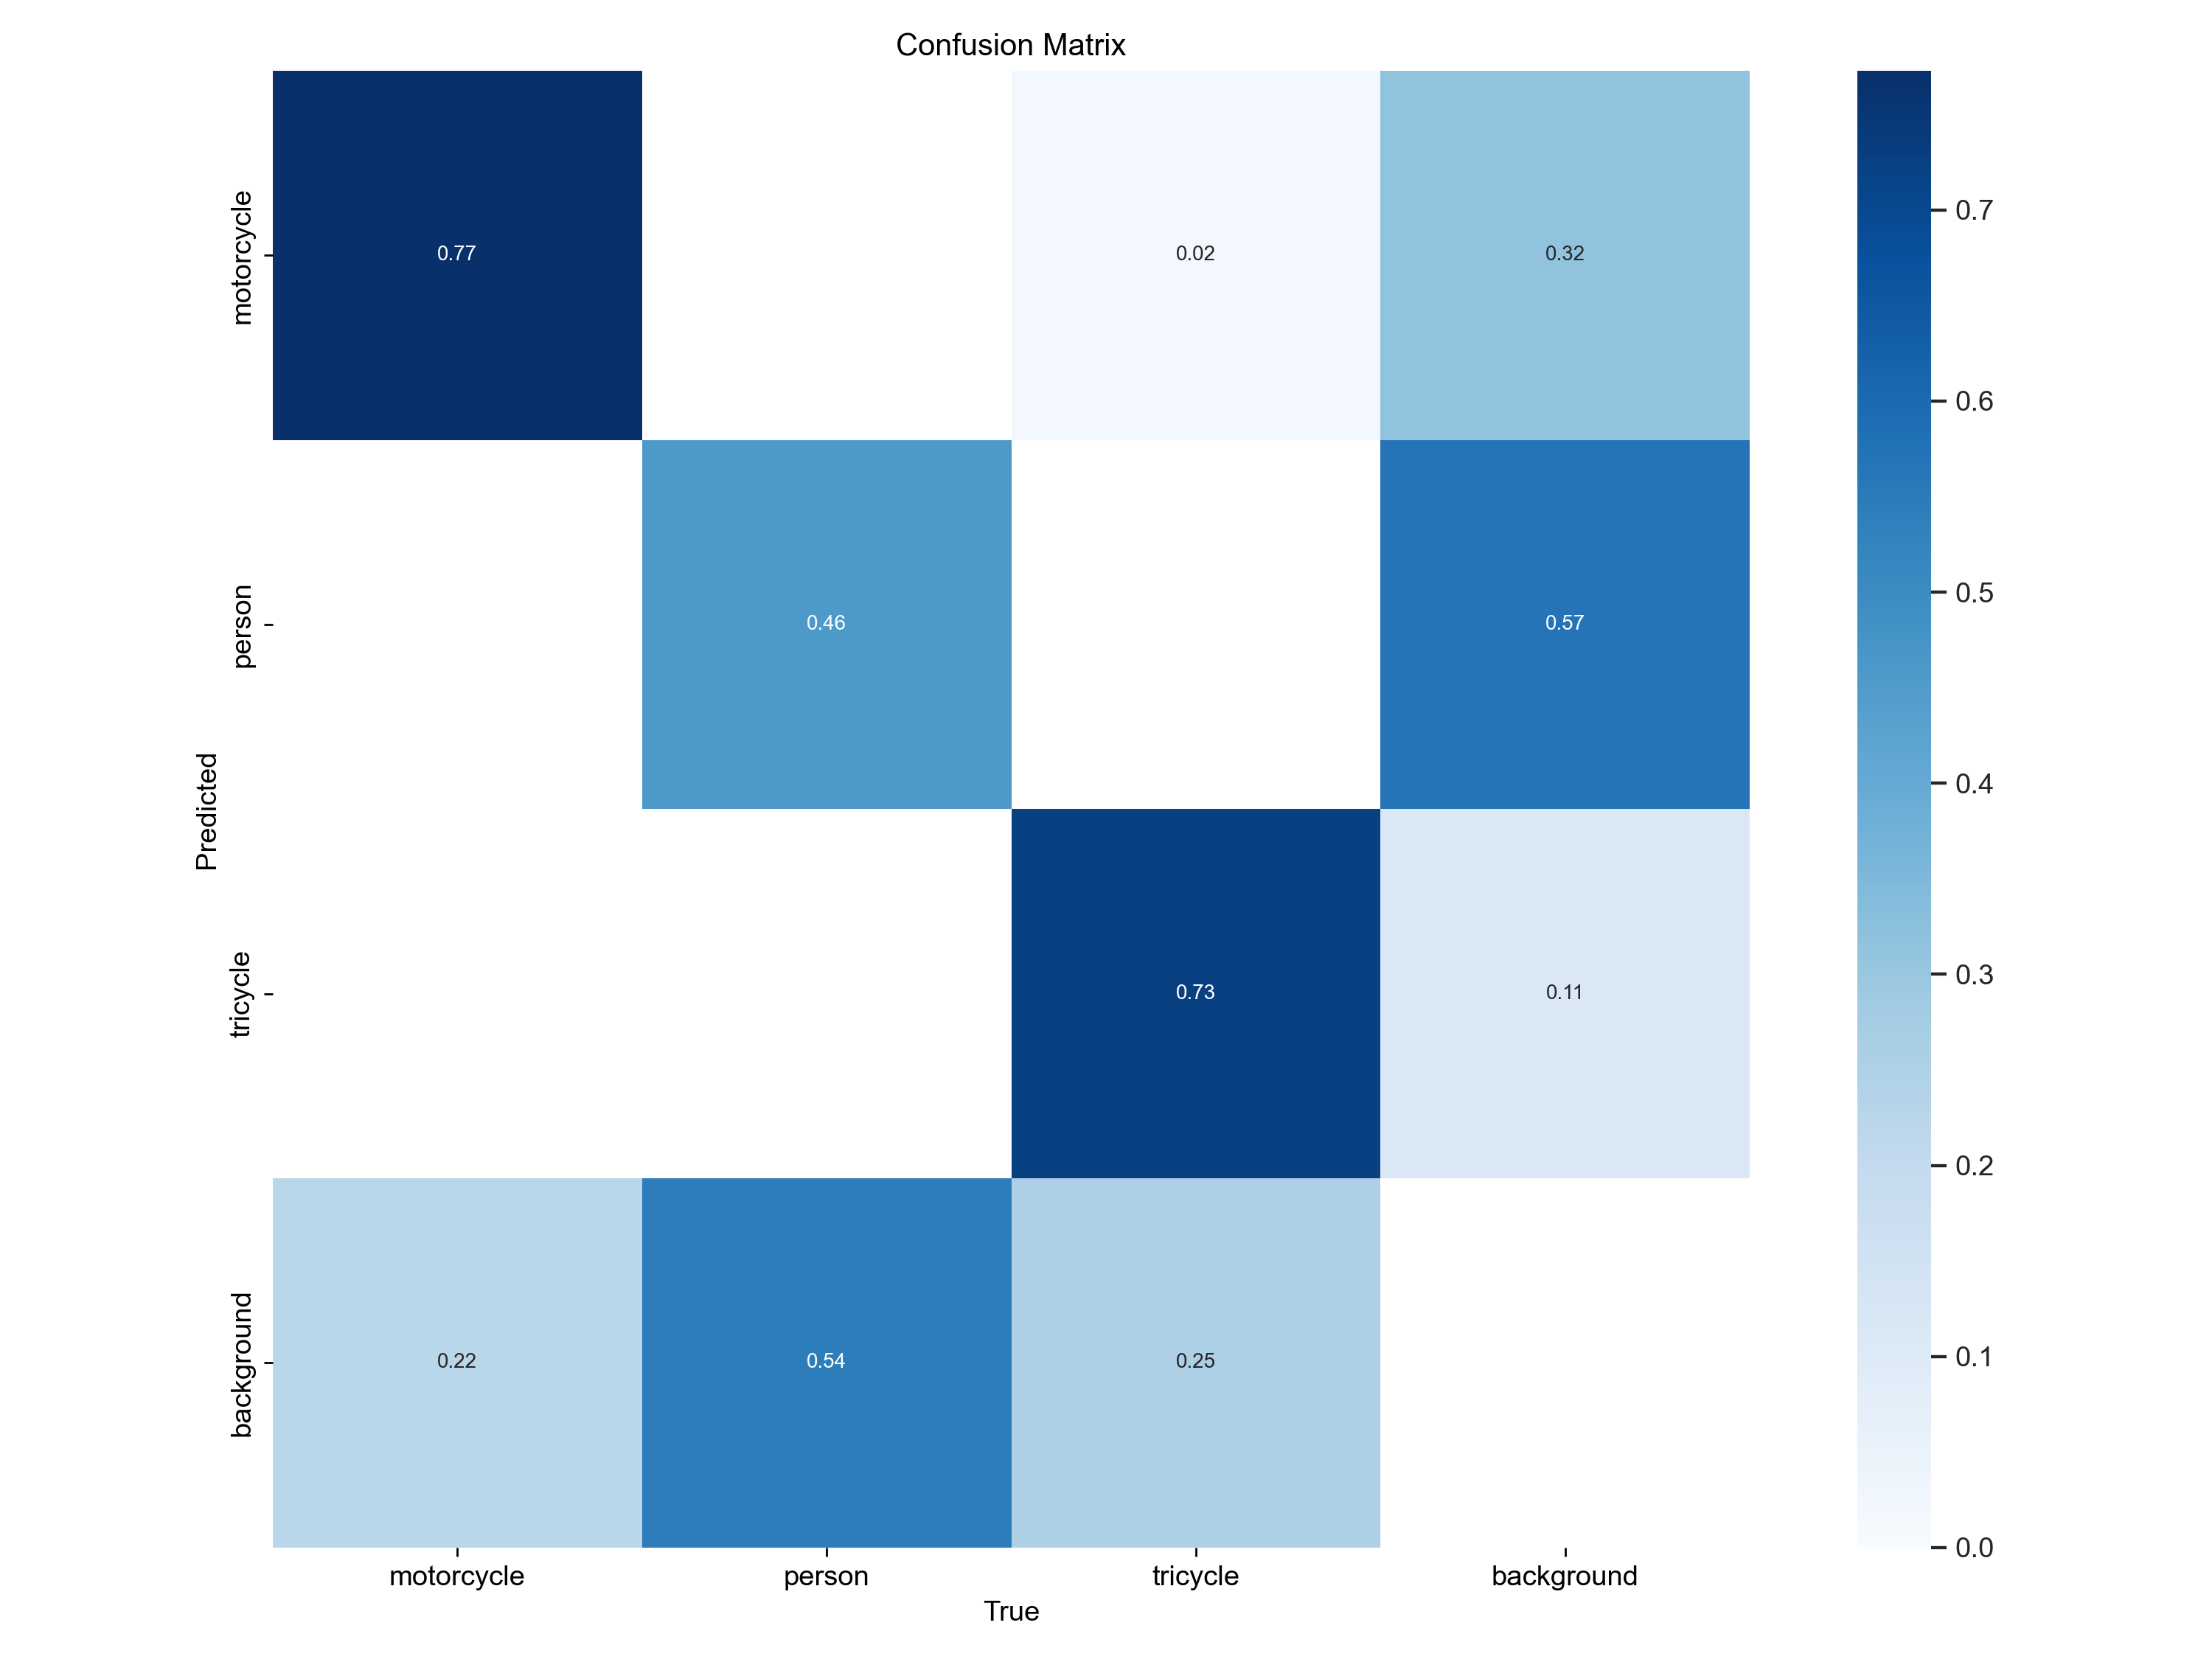
\includegraphics[width=\columnwidth]{Figures/dataset_b/b_confusion_matrix.png}
			\caption{Dataset B: Confusion Matrix of YOLOv5 model}
			\label{fig:mtpDatasetYolov5LargeWeight}
		\end{figure}

		\begin{figure}[h]
			\centering
			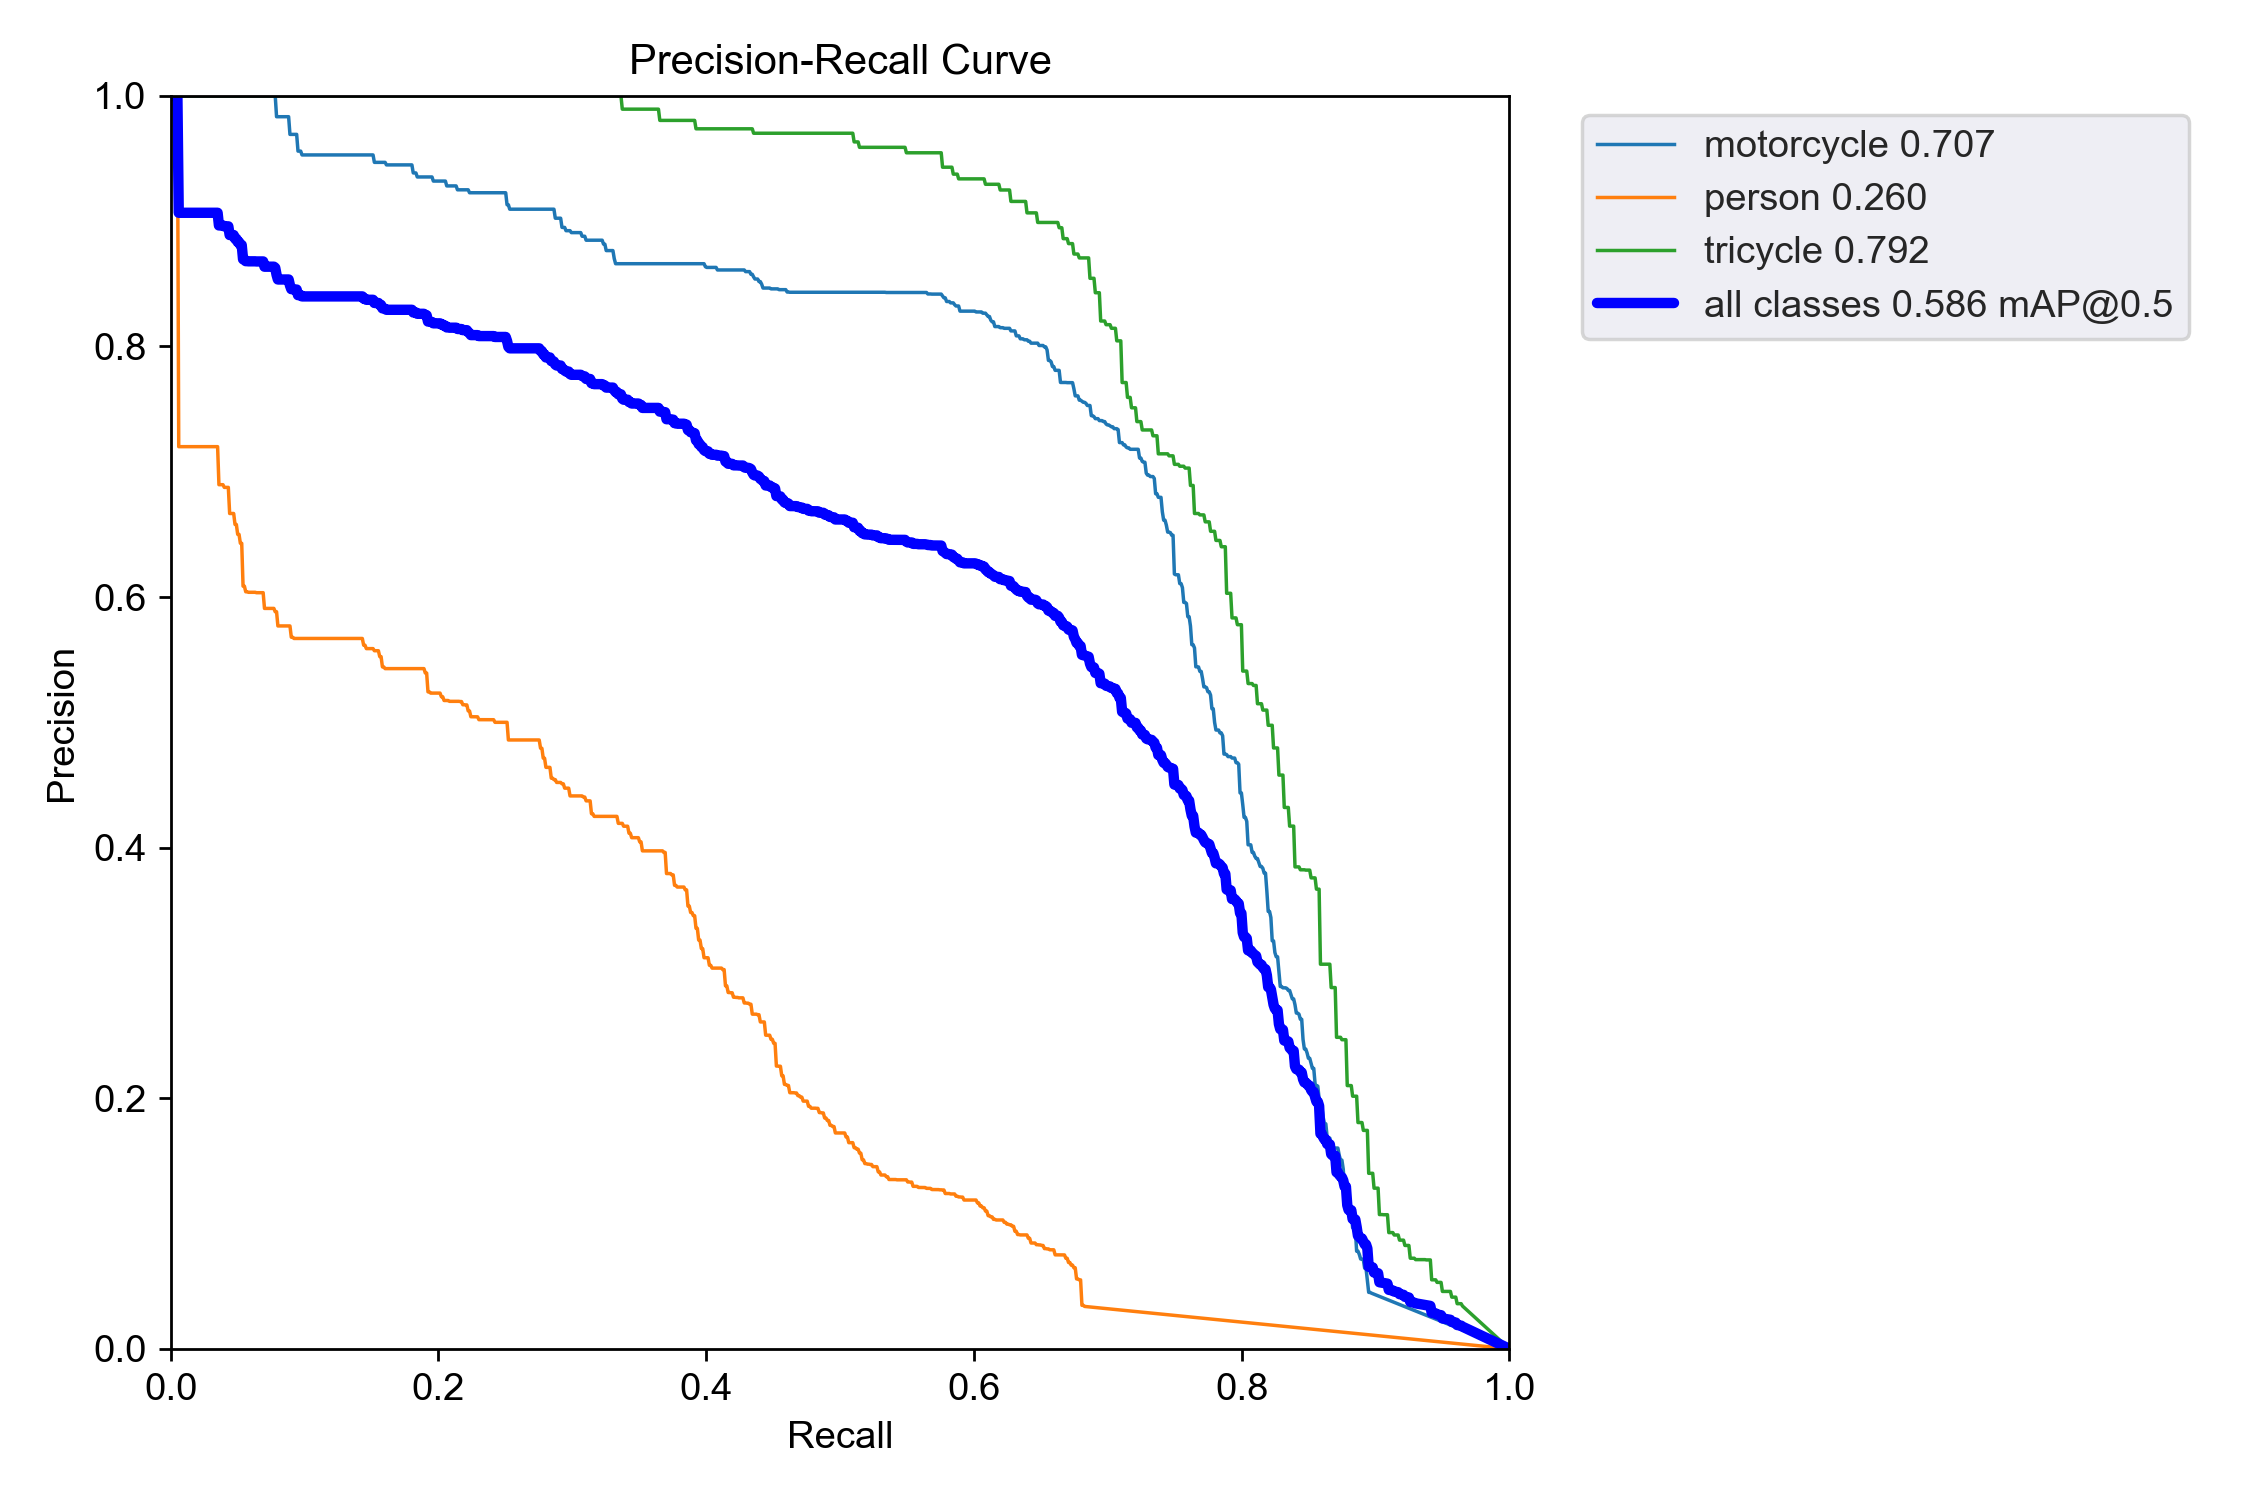
\includegraphics[width=\columnwidth]{Figures/dataset_b/PR_curve.png}
			\caption{Dataset B: Performance and Recall of YOLOv5 model}
			\label{fig:mtpDatasetYolov5LargeWeightPRCurve}
		\end{figure}

\section{Current Findings}
	The following images of~\ref{fig:detectionOfMotorcycleW1},~\ref{fig:detectionOfMotorcycleW2} and~\ref{fig:detectionOfMotorcycleW3} show different wet condition scenarios. Due to previous research conducted, according to Tesla, ``Tesla announces in 2021 that the company would remove a sensor called Ultrasonic Sensors, replacing the sensor with `Tesla Vision' by 2022''.~\cite{noauthor_tesla_nodate} This only means according to ``Self-Driving Cars and The Law: Putting autonomous vehicles on the road isn't just a matter of fine-tuning technology'' by Nathan A. Greenblatt, that AVs used `...thanks to lidar, radar, and ultrasonic sensors, they can see through fog and in the dark.', meaning that Tesla AVs for example, only use a visual aid to see. However, this raises concerns about the reliability of AVs solely using visual input. In situations where the camera's view is obscured by wet patches or heavy fog, a human driver could outperform the technology.

	Figure~\ref{fig:detectionOfMotorcycleW1} of a motorcycle in wet weather conditions, the architecture trained weight has successfully found the motorcycle with 75\% positiveness that it is a motorcycle.

	Figure~\ref{fig:detectionOfMotorcycleW2} of a motorcycle in wet weather conditions, the architecture failed to find the motorcycle. This scenario happened when the water content blurred the camera, which could simulate current problems with vision technology within AVs.

	Figure~\ref{fig:detectionOfMotorcycleW3} of a motorcycle in wet weather conditions, the architecture failed to find the motorcycle. The visibility is moderate; human eyesight can easily see more than eight to ten meters ahead. Another observation of this footage was that the vehicles are visible, although the architecture failed to recognise the motorcycle.
	\begin{figure}[h]
		\centering
		\begin{minipage}{0.15\textwidth}
			\centering
			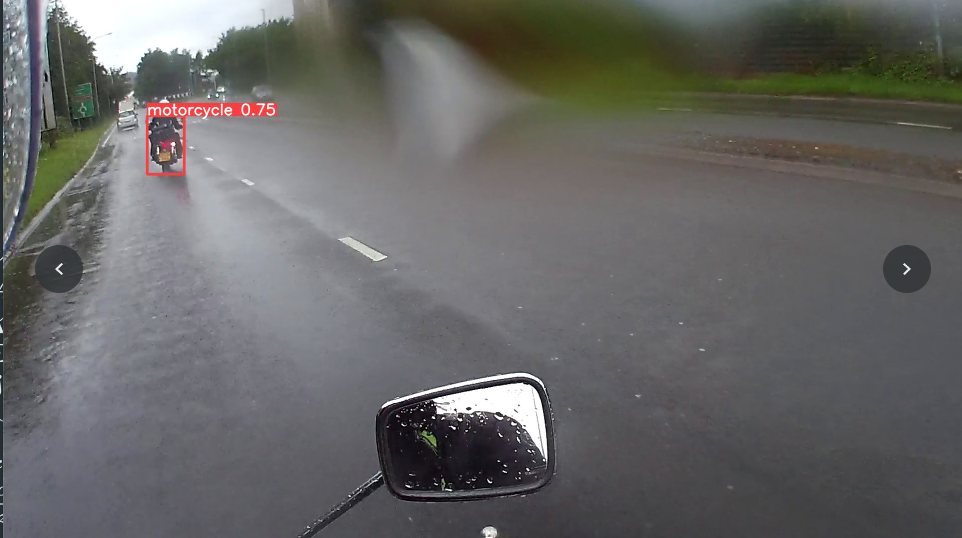
\includegraphics[width=\linewidth]{Figures/wet_correct.png}
			\caption{Good Detection of Motorcycle - Wet and Multi Lane}
			\label{fig:detectionOfMotorcycleW1}
		\end{minipage}\hfill
		\begin{minipage}{0.15\textwidth}
			\centering
			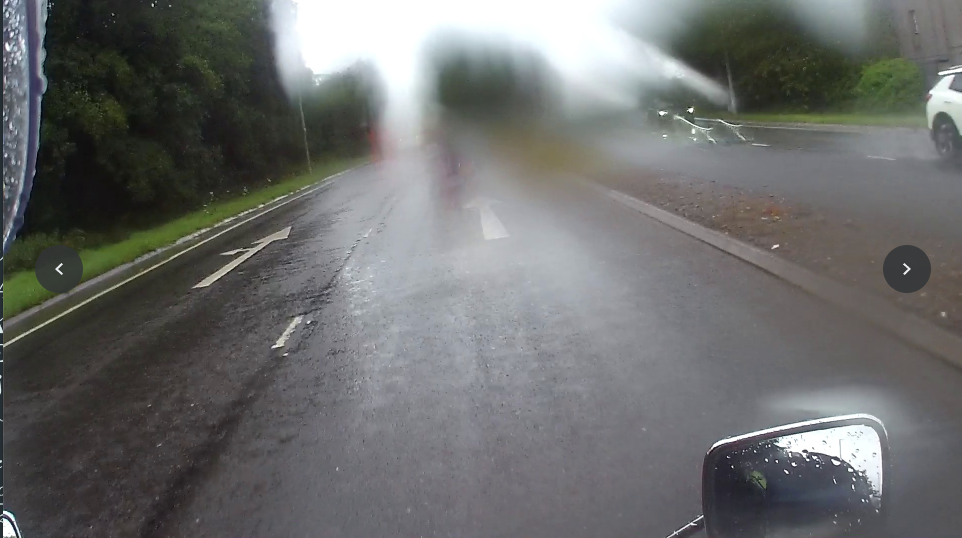
\includegraphics[width=\linewidth]{Figures/wet_incorrect.png}
			\caption{Classification Error - Camera Blinded}
			\label{fig:detectionOfMotorcycleW2}
		\end{minipage}\hfill
		\begin{minipage}{0.15\textwidth}
			\centering
			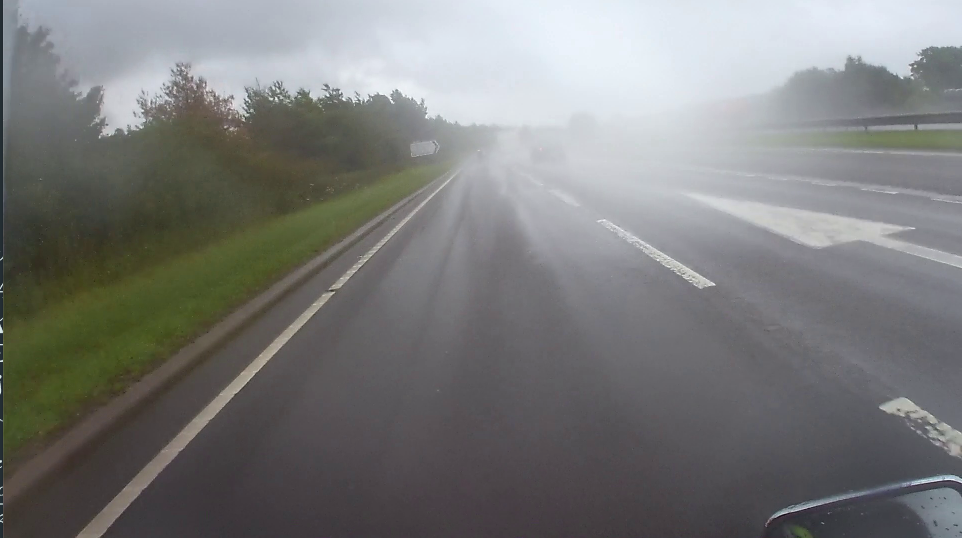
\includegraphics[width=\linewidth]{Figures/wet_danger.png}
			\caption{Classification Error - Water Spray from Other Vehicles}
			\label{fig:detectionOfMotorcycleW3}
		\end{minipage}
	\end{figure}	

    Figure~\ref{fig:detectionOfOneMotorcycle} of detecting one motorcycle may not seem dangerous. However, if an AV misclassifies or does not detect the motorcycle after the first motorcycle, the AV may not be able to foresee any sudden traffic actions, causing fatal collisions.

    Figures~\ref{fig:lateClassificationP1},~\ref{fig:lateClassificationP2} demonstrates the dangers of motorcycle misclassification near a junction. If the AV were to turn right, coming out of the junction, then due to the AV not anticipating the motorcyclist, then the AV may pull out on the motorcycle, causing a fatality. The Object Classification did, however, detect the motorcycle when it was closer to the motorcycle.
	\begin{figure}[h]
		\centering
		\begin{minipage}{0.15\textwidth}
			\centering
			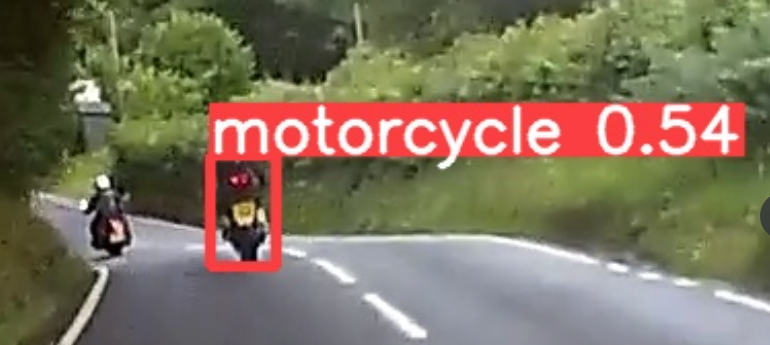
\includegraphics[width=\linewidth]{Figures/fail.png}
			\caption{Detection of One Motorcycle}
			\label{fig:detectionOfOneMotorcycle}
		\end{minipage}\hfill
		\begin{minipage}{0.15\textwidth}
			\centering
			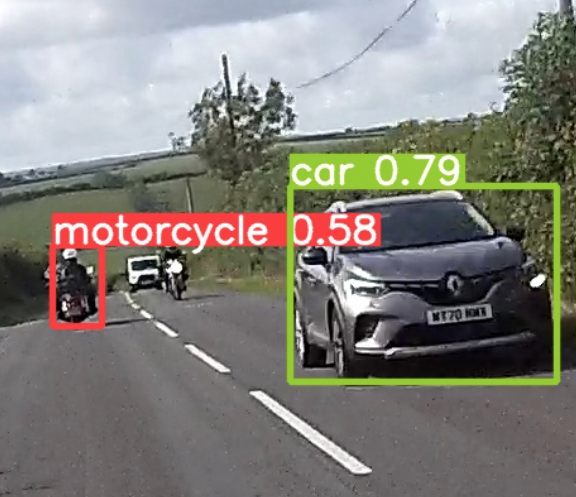
\includegraphics[width=\linewidth]{Figures/left_turn.png}
			\caption{Late Classification - Part 1}
			\label{fig:lateClassificationP1}
		\end{minipage}\hfill
		\begin{minipage}{0.15\textwidth}
			\centering
			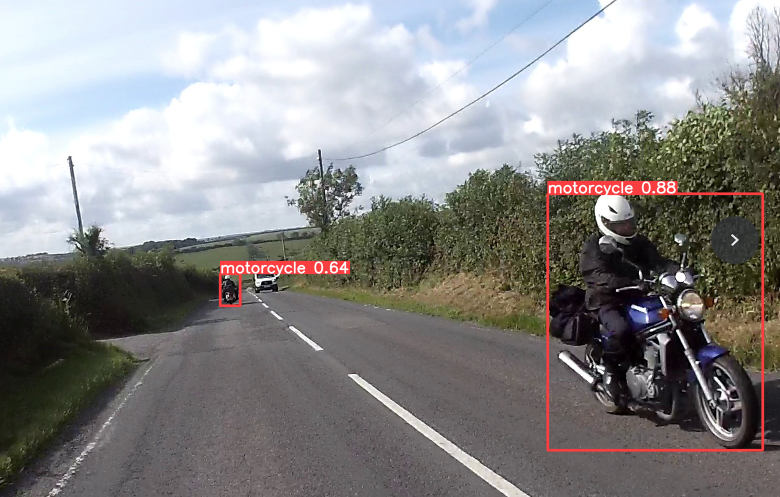
\includegraphics[width=\linewidth]{Figures/motorcycle.png}
			\caption{Late Classification - Part 2}
			\label{fig:lateClassificationP2}
		\end{minipage}
	\end{figure}	

	Figure~\ref{fig:overtakingSequence} shows a 75\% accuracy of correctly identifying two motorcycles after two overtakes. However, the last sequence shows an overtaking procedure involving two tractors and two motorcycles. The classification process is concerning, considering the motorcycles were not detected. This concern arises from a few things, the AV could perform an overtaking manoeuvre and accelerate unsafely, or if an AV started approaching at the speed limit, the AV might not slow down, even though other traffic is overtaking behind the riders to get by tractors safely.
	\begin{figure}[h]
		\centering
		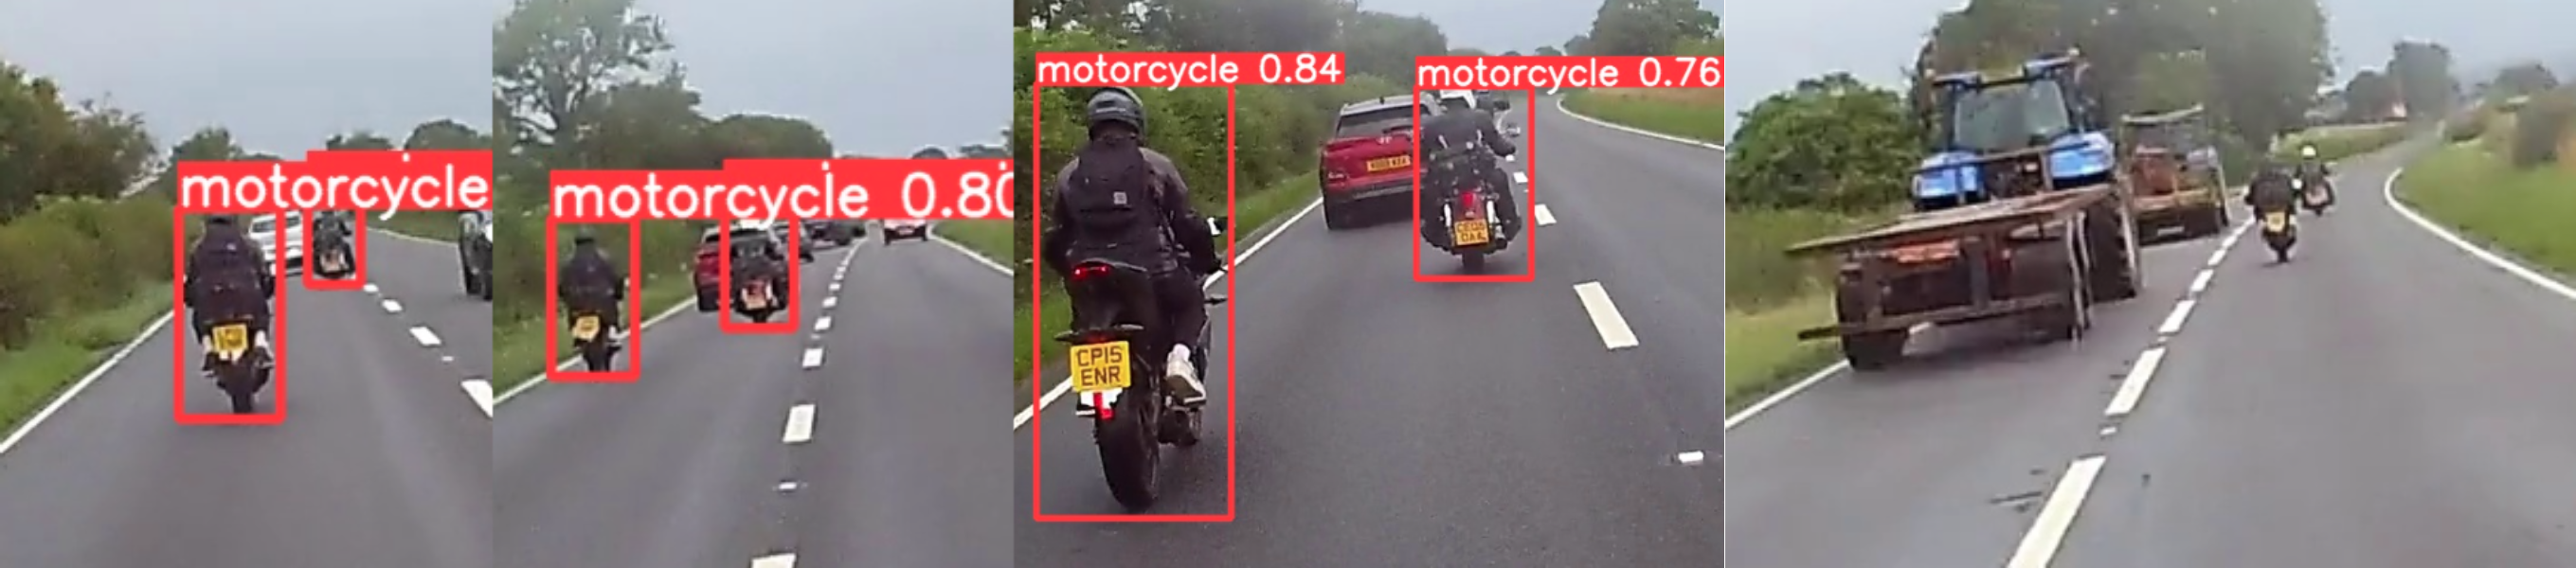
\includegraphics[width=\columnwidth]{Figures/motorcycle_overtaking_sequence.png}
		\caption{Overtaking Sequence}
		\label{fig:overtakingSequence}
	\end{figure}
\section{Discussion}
	\subsection{Training Sequence}
	The trained classification uses Asian and US footage to train the model. According to the classification models found in figures (\ref{fig:ukDatasetYolov5LargeWeight}~\ref{fig:mtpDatasetYolov5LargeWeight}), the motorcycle had an 81\% accuracy within fig~\ref{fig:ukDatasetYolov5LargeWeight}, with 39\% outliers identifying motorcycle objects as Scooters, with a minimal of 15\% outliers identifying as background. In comparison to the Motorcycle, Trike and Person model, found in fig~\ref{fig:mtpDatasetYolov5LargeWeight}, the motorcycle had a 77\% accuracy, with 32\% of outliers identifying as background.

    Figures (\ref{fig:ukDatasetYolov5LargeWeightPRCurve}~\ref{fig:mtpDatasetYolov5LargeWeightPRCurve}) show the Precision and Recall curves plotted on a graph, giving information on any performance issues with the training models. The PR curves for both models demonstrate high precision across varying levels of recall, indicative of robust performance. Although, figure~\ref{fig:ukDatasetYolov5LargeWeightPRCurve} appears to have a higher precision for the longer part of the training process, compared to figure~\ref{fig:mtpDatasetYolov5LargeWeightPRCurve}. The worse performers of the model are scooters, vans, person and minivans in precision and perform well when it comes to recall. In comparison, figure~\ref{fig:mtpDatasetYolov5LargeWeightPRCurve} shows a similar illustration. According to the key of figure~\ref{fig:ukDatasetYolov5LargeWeightPRCurve}, motorcycles had a higher precision peak at 77.5\% compared to figure~\ref{fig:mtpDatasetYolov5LargeWeightPRCurve}. The model architecture performs well when training the given dataset scenarios. Perhaps larger weights could increase the precision and recall curve during training. It is worth mentioning that the preparation of the datasets functions well during the training process, and no underlying problems are showing, especially for motorcycle data.

	During the testing sequence, the larger trained model was selected. Arguably, the 81\% accuracy for motorcycles, with 39\% outliers identifying as scooters or even a 3\% as a trike, is still safer than having most motorcycles identified as background objects. The accuracy of this training may come under a few situations, including better object classification training material for motorcycles, especially in foggy, wet, overtaking and filtering situations within the UK. It is also important to note that gathering and publishing such materials publicly in Britain could infringe the Data Protection Act 2018 (...meeting the standards to the EU GDPR guidelines)~\cite{govuk_data_2018} law, including but not limited to:

		\begin{itemize}
			\item Must inform the member of public how the data is being used.
			\item Must allow the member of public to access personal data.
			\item Must have incorrect data updated. - This is important for the member of public to access personal data.
			\item Must allow the member of public to erase data. Which can impede the training process in one way or another.
			\item The member of public has right to stop or restrict processing of your data. - Which impacts the training process.
			\item Data portability, to allow the data to be used for different purposes.
			\item Member of public has rights to object to how your data is processed in certain situations.
		\end{itemize}

		Furthermore, member of the public has rights when it comes to automated decision-making processes (without human involvement), which could suggest Machine Learning purposes, and profiling, to predict behaviour or interests. These all matter regarding British legislation and could impede AVs from being trained in the UK when fetching video data from pedestrians, cyclists, car drivers and other motorists. This finding could indicate the lack of public datasets available for motorcyclists or any other vehicles in the UK, complicating the training process.

	\subsection{Testing Sequence}
		A few issues come to light after running through the gathered test results. The footage involves mixed scenarios including wet, dry and overtaking procedures. There is a few prospectives that need addressing when observing the test footage. Before going into a deeper level of understanding why accurate classifications are important, and it does not stop at detecting a motorcycle, as hand gestures, and person's bodies are equally important, when it comes to indicating, warning they are braking, or if a fortunate accident were to happen, including a pillion (passenger of the vehicle) or operator was to suddenly come off in the road. A important emphasis would include, would the AV detect this, or would it only register the motorcycle still riding in a straightline, causing the AV not to stop, avoiding potential death. 
		
		The Ministry of Transport (MOT) has different requirements for a motorcycle. Motorcycles can potentially lack of headlamps, main beam, and offers a range of colours; white, yellow and mainly white light with a blue tinge. Direction indicators are not required to pass the MOT, if the said vehicle, in-particular, `do not have front and rear position lamps'. However, there is other exemptions too. Motorcycles electronics are not always reliable, in some cases, riders accept this `risk', and even though it is stated a `Minor', `Major' to `Dangerous' categories on the MOT, motorcycles may use hand signals to communicate to other road users that the vehicle is slowing down. That said, this is a common practice we are taught as British road users, if any indication equipment goes wrong to keep the vehicles on the road safe. These are things the British road users deal with sub-conciously, and AVs should be expected to have understanding of the road safety rulings, especially when it comes to more vulnerable users such as motorcyclists, cyclists, and horse riders.
		
		In figures (\ref{fig:detectionOfMotorcycleW1}~\ref{fig:detectionOfMotorcycleW2}~\ref{fig:detectionOfMotorcycleW3}) display three scenarios. A problem that is evident is the camera used kept getting water on, so the camera used in AVs have to have resilliance to repel water in order to remain safe on the road. However, the camera fails to pick up the motorcycle in figure~\ref{fig:detectionOfMotorcycleW3}, showing the importance of noting that not all motorcycles may have their lights on, in this case the light is on. However, fog lights were not required, so even having any sort of implementation on the vehicle would not help, as it was not the right conditions for the given scenario, and could cause blindness and eye-fatigue to other road users.

		In figures (\ref{fig:detectionOfOneMotorcycle}~\ref{fig:lateClassificationP1}~\ref{fig:lateClassificationP2}) displays the importantance of safety when rolling out AVs within the UK. The detection of motorcycles seems to be limited, however, with some sort of tracking implementation when detection is detected it could help the process. Although, tracking doesn't gurantee the motorcycles are always in sight. A common theme found when performing these detections, is when a motorcycle started to be further in the distance detection was useless. This leads to figure~\ref{fig:lateClassificationP1} and~\ref{fig:lateClassificationP2} where the on-coming motorcycle was not immediately detected, and if for some reason the AV had to make a right turn or a swerve to the right, rather than applying the braking system, then the misunfortunate rider would have zero to no time to react the intention of the AV.

		% mention fog lights and safety features
		
\section{Conclusion}

\section{Further Research}
	The increasing prevalence of AVs on the roads presents a wide array of challenges and questions, particularly when it comes to their interactions with vulnerable road users like motorcyclists. The mentioned questions and concerns provide an excellent starting point for further research. Here's a deeper dive into the potential areas of research:

	\begin{enumerate}
		\item Emergency Braking Systems and Motorcycles:
		\begin{itemize}
			\item How do AVs' emergency braking systems currently detect and react to motorcycles?
			\item What circumstances could lead an AV to detect a motorcycle late, necessitating emergency braking?
			\item Does the size, speed, or color of the motorcycle affect detection?
		\end{itemize}
		\item Blindspot Detection and Mitigation:
		\begin{itemize}
			\item To what extent do AVs recognize motorcycles in their blindspots?
			\item How does the AV's software differentiate between a motorcycle and other vehicles or objects in its blindspot?
			\item What are the current solutions to this problem, and how effective are they?
		\end{itemize}
		\item Behavioral Adaptations by Motorcyclists:
		\begin{itemize}
			\item How can motorcyclists adapt their riding behaviour to ensure safety as AVs become prevalent on UK roads?
			\item What education or training can be provided to motorcyclists regarding AV behaviour?
			\item Are there specific manoeuvres or positions that motorcyclists should adopt or avoid when in the vicinity of an AV?
		\end{itemize}
		\item Night and Fog Driving:
		\begin{itemize}
			\item How do AV sensors and software handle low-visibility conditions, such as night driving or fog, especially without LiDAR technology?
			\item Given their smaller size and potentially reduced visibility, are there specific challenges posed by motorcycles under these conditions?
			\item How do current AV systems compare regarding their effectiveness in these conditions?
		\end{itemize}

		\item Safety Protocols for New Market Entrants:
		\begin{itemize}
			\item As more companies enter the AV market, what safety protocols or standards exist regarding motorcycle detection and safe management?
			\item How can regulatory bodies ensure that new entrants prioritize the safety of motorcyclists in their software and hardware development?
		\end{itemize}
	\end{enumerate}

	Given the potential ramifications of a collision between an AV and a motorcycle or other vulnerable road users, it is paramount that these questions be addressed thoroughly. Research in this area not only contributes to the academic community but also has the potential to inform public policy, industry standards, and public education efforts.

\section{Terminology}
	List of terminologies used in this document:-
	\begin{itemize}
		\item AV - Autonomous Vehicles.
		\item LiDAR - Light Detection and Ranging.
		\item MOT - Ministry of Transport.
	\end{itemize}

\nocite{*}
\renewcommand\refname{\section{Reference List}}
\small{\bibliographystyle{IEEEtran}
	\bibliography{ref}}
\end{document}